\documentclass[10pt]{beamer}
\usepackage[english]{babel}
\usepackage[utf8]{inputenc}
\usepackage[T1]{fontenc}
\usepackage{helvet}

%-------------------------------------------------------
% INFORMATION IN THE TITLE PAGE
%-------------------------------------------------------

\newcommand{\cstitle}{\textbf{Desarrollo de una aplicación Web para la detección de neoantígenos en el marco de desarrollo de vacunas personalizadas para tratar el Cáncer}}
\subtitle[]{Proyecto interno de la universidad}
\newcommand{\cscourseCode}{Neoantígenos}
\newcommand{\csauthor}{Dr. Vicente Machaca Arceda \\ Mg. Richart Escobedo \\ Jose Grados \\ Kristhyan Lazarte}
\institute[UNSA]{Universidad La Salle}
\newcommand{\csemail}{vmachaca@utec.edu.pe}
\newcommand{\instituteabr}{UTEC}
\newcommand{\nameUp}{}
\date{2024}
\title[\cscourseCode]{\cstitle}
\author{\csauthor}
%%%%%%%%%%%%%%%%%

%-------------------------------------------------------
% CHOOSE THE THEME
%-------------------------------------------------------
\def\mycmd{0} % UNSA
\def\mycmd{1} % SALLE
%\def\mycmd{2} % UTEC
%-------------------------------------------------------

\if\mycmd0
\usepackage{csformat}
\newcommand{\chref}[3][blue]{\href{#2}{\color{#1}{#3}}}%

\fi

\if\mycmd1
\usetheme[]{Feather}
\newcommand{\chref}[2]{	\href{#1}{{\usebeamercolor[bg]{Feather}#2}} }
\fi

\if\mycmd2
\usetheme{UTEC2020}	
\newcommand{\chref}[3][blue]{\href{#2}{\color{#1}{#3}}}%
\fi

\newcommand{\1}{
	\setbeamertemplate{background}{
		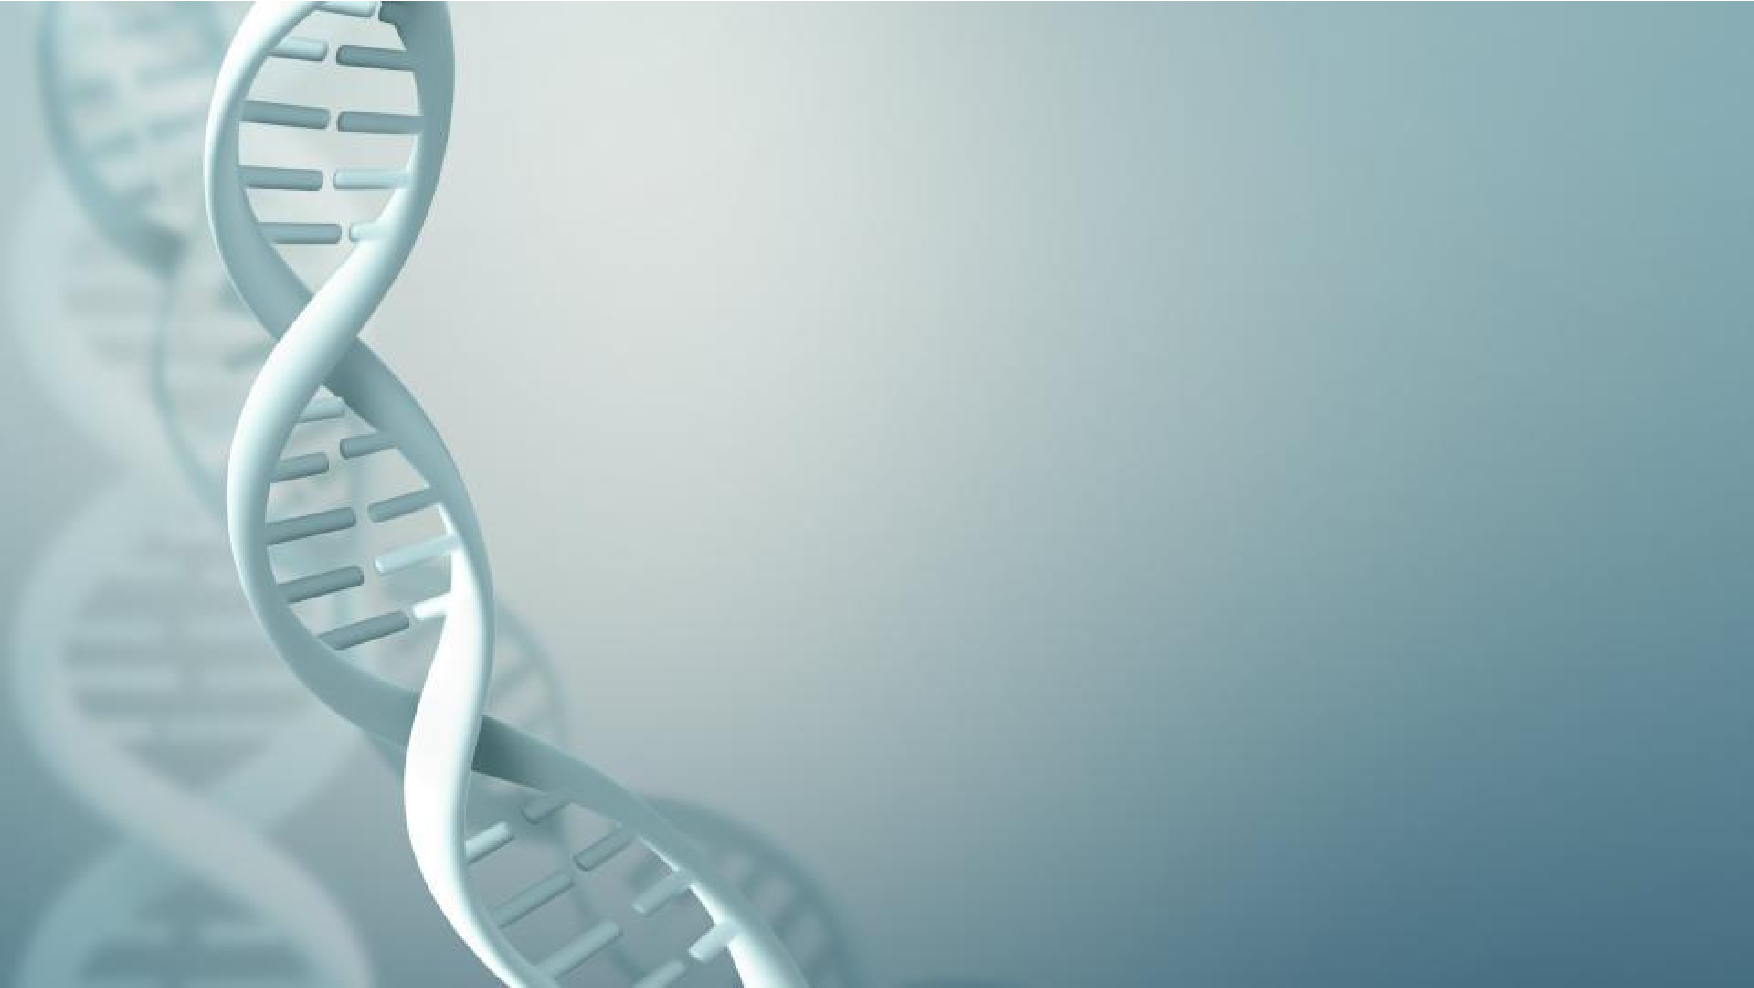
\includegraphics[width=\paperwidth,height=\paperheight]{../img/1}
		\tikz[overlay] \fill[fill opacity=0.75,fill=white] (0,0) rectangle (-\paperwidth,\paperheight);
	}
}



%-------------------------------------------------------
% THE BODY OF THE PRESENTATION
%-------------------------------------------------------

\begin{document}
	
	
	\AtBeginSection[]
	{
		\begin{frame}
			\frametitle{Contenido}
			\tableofcontents[currentsubsection]
		\end{frame}
	}
	
	
	%-------------------------------------------------------
	% THE TITLEPAGE
	%-------------------------------------------------------
	
	\if\mycmd0
	\maketitle
	\fi
	
	\if\mycmd1 % MY THEME
	\1{
		\begin{frame}[plain,noframenumbering] 
			\titlepage 
	\end{frame}}
	\fi
	
	\if\mycmd2
	\begin{frame}
		\titlepage
	\end{frame}
	\fi
	%-------------------------------------------------------
	%-------------------------------------------------------
	
	
	%-------------------------------------------------------
	%-------------------------------------------------------
	\begin{frame}{Contenido}
		\tableofcontents
	\end{frame}
	%-------------------------------------------------------
	%-------------------------------------------------------
	
	
	%%%%%%%%%%%%%%%%%%%%%%%%%%%%%%%%%%%%%%%%%%%%%%%%%%%%%%%%%%%%%%%%%%%%%%%%%%%%%%%%%%%%%%%%%%%%%%%%%%%%%%%%%%%%%%%%
	%%%%%%%%%%%%%%%%%%%%%%%%%%%%%%%%%%%%%%%%%%%%%%%%%%%%%%%%%%%%%%%%%%%%%%%%%%%%%%%%%%%%%%%%%%%%%%%%%%%%%%%%%%%%%%%%
	%%%%%%%%%%%%%%%%%%%%%%%%%%%%%%%%%%%%%%%%%%%%%%%%%%%%%%%%%%%%%%%%%%%%%%%%%%%%%%%%%%%%%%%%%%%%%%%%%%%%%%%%%%%%%%%%
	\section{Marco teórico}
	%%%%%%%%%%%%%%%%%%%%%%%%%%%%%%%%%%%%%%%%%%%%%%%%%%%%%%%%%%%%%%%%%%%%%%%%%%%%%%%%%%%%%%%%%%%%%%%%%%%%%%%%%%%%%%%%
	%%%%%%%%%%%%%%%%%%%%%%%%%%%%%%%%%%%%%%%%%%%%%%%%%%%%%%%%%%%%%%%%%%%%%%%%%%%%%%%%%%%%%%%%%%%%%%%%%%%%%%%%%%%%%%%%
	%%%%%%%%%%%%%%%%%%%%%%%%%%%%%%%%%%%%%%%%%%%%%%%%%%%%%%%%%%%%%%%%%%%%%%%%%%%%%%%%%%%%%%%%%%%%%%%%%%%%%%%%%%%%%%%%
	
	%%%%%%%%%%%%%%%%%%%%%%%%%%%%%%%%%%%%%%%%%%%%%%%%%%%%%%%%%%%%%%%%%%%%%%%%%%%%%%%%%%%%%%%%%%%%%%%%%%%%%%%%%%%%%%%%
	%%%%%%%%%%%%%%%%%%%%%%%%%%%%%%%%%%%%%%%%%%%%%%%%%%%%%%%%%%%%%%%%%%%%%%%%%%%%%%%%%%%%%%%%%%%%%%%%%%%%%%%%%%%%%%%%
	%%%%%%%%%%%%%%%%%%%%%%%%%%%%%%%%%%%%%%%%%%%%%%%%%%%%%%%%%%%%%%%%%%%%%%%%%%%%%%%%%%%%%%%%%%%%%%%%%%%%%%%%%%%%%%%%
	\subsection{Bioinformática y DNA}
	%%%%%%%%%%%%%%%%%%%%%%%%%%%%%%%%%%%%%%%%%%%%%%%%%%%%%%%%%%%%%%%%%%%%%%%%%%%%%%%%%%%%%%%%%%%%%%%%%%%%%%%%%%%%%%%%
	%%%%%%%%%%%%%%%%%%%%%%%%%%%%%%%%%%%%%%%%%%%%%%%%%%%%%%%%%%%%%%%%%%%%%%%%%%%%%%%%%%%%%%%%%%%%%%%%%%%%%%%%%%%%%%%%
	%%%%%%%%%%%%%%%%%%%%%%%%%%%%%%%%%%%%%%%%%%%%%%%%%%%%%%%%%%%%%%%%%%%%%%%%%%%%%%%%%%%%%%%%%%%%%%%%%%%%%%%%%%%%%%%%
	

	
	%-------------------------------------------------------
	%-------------------------------------------------------
	\begin{frame}{DNA}{Localización}
		\begin{figure}[]
			\centering
			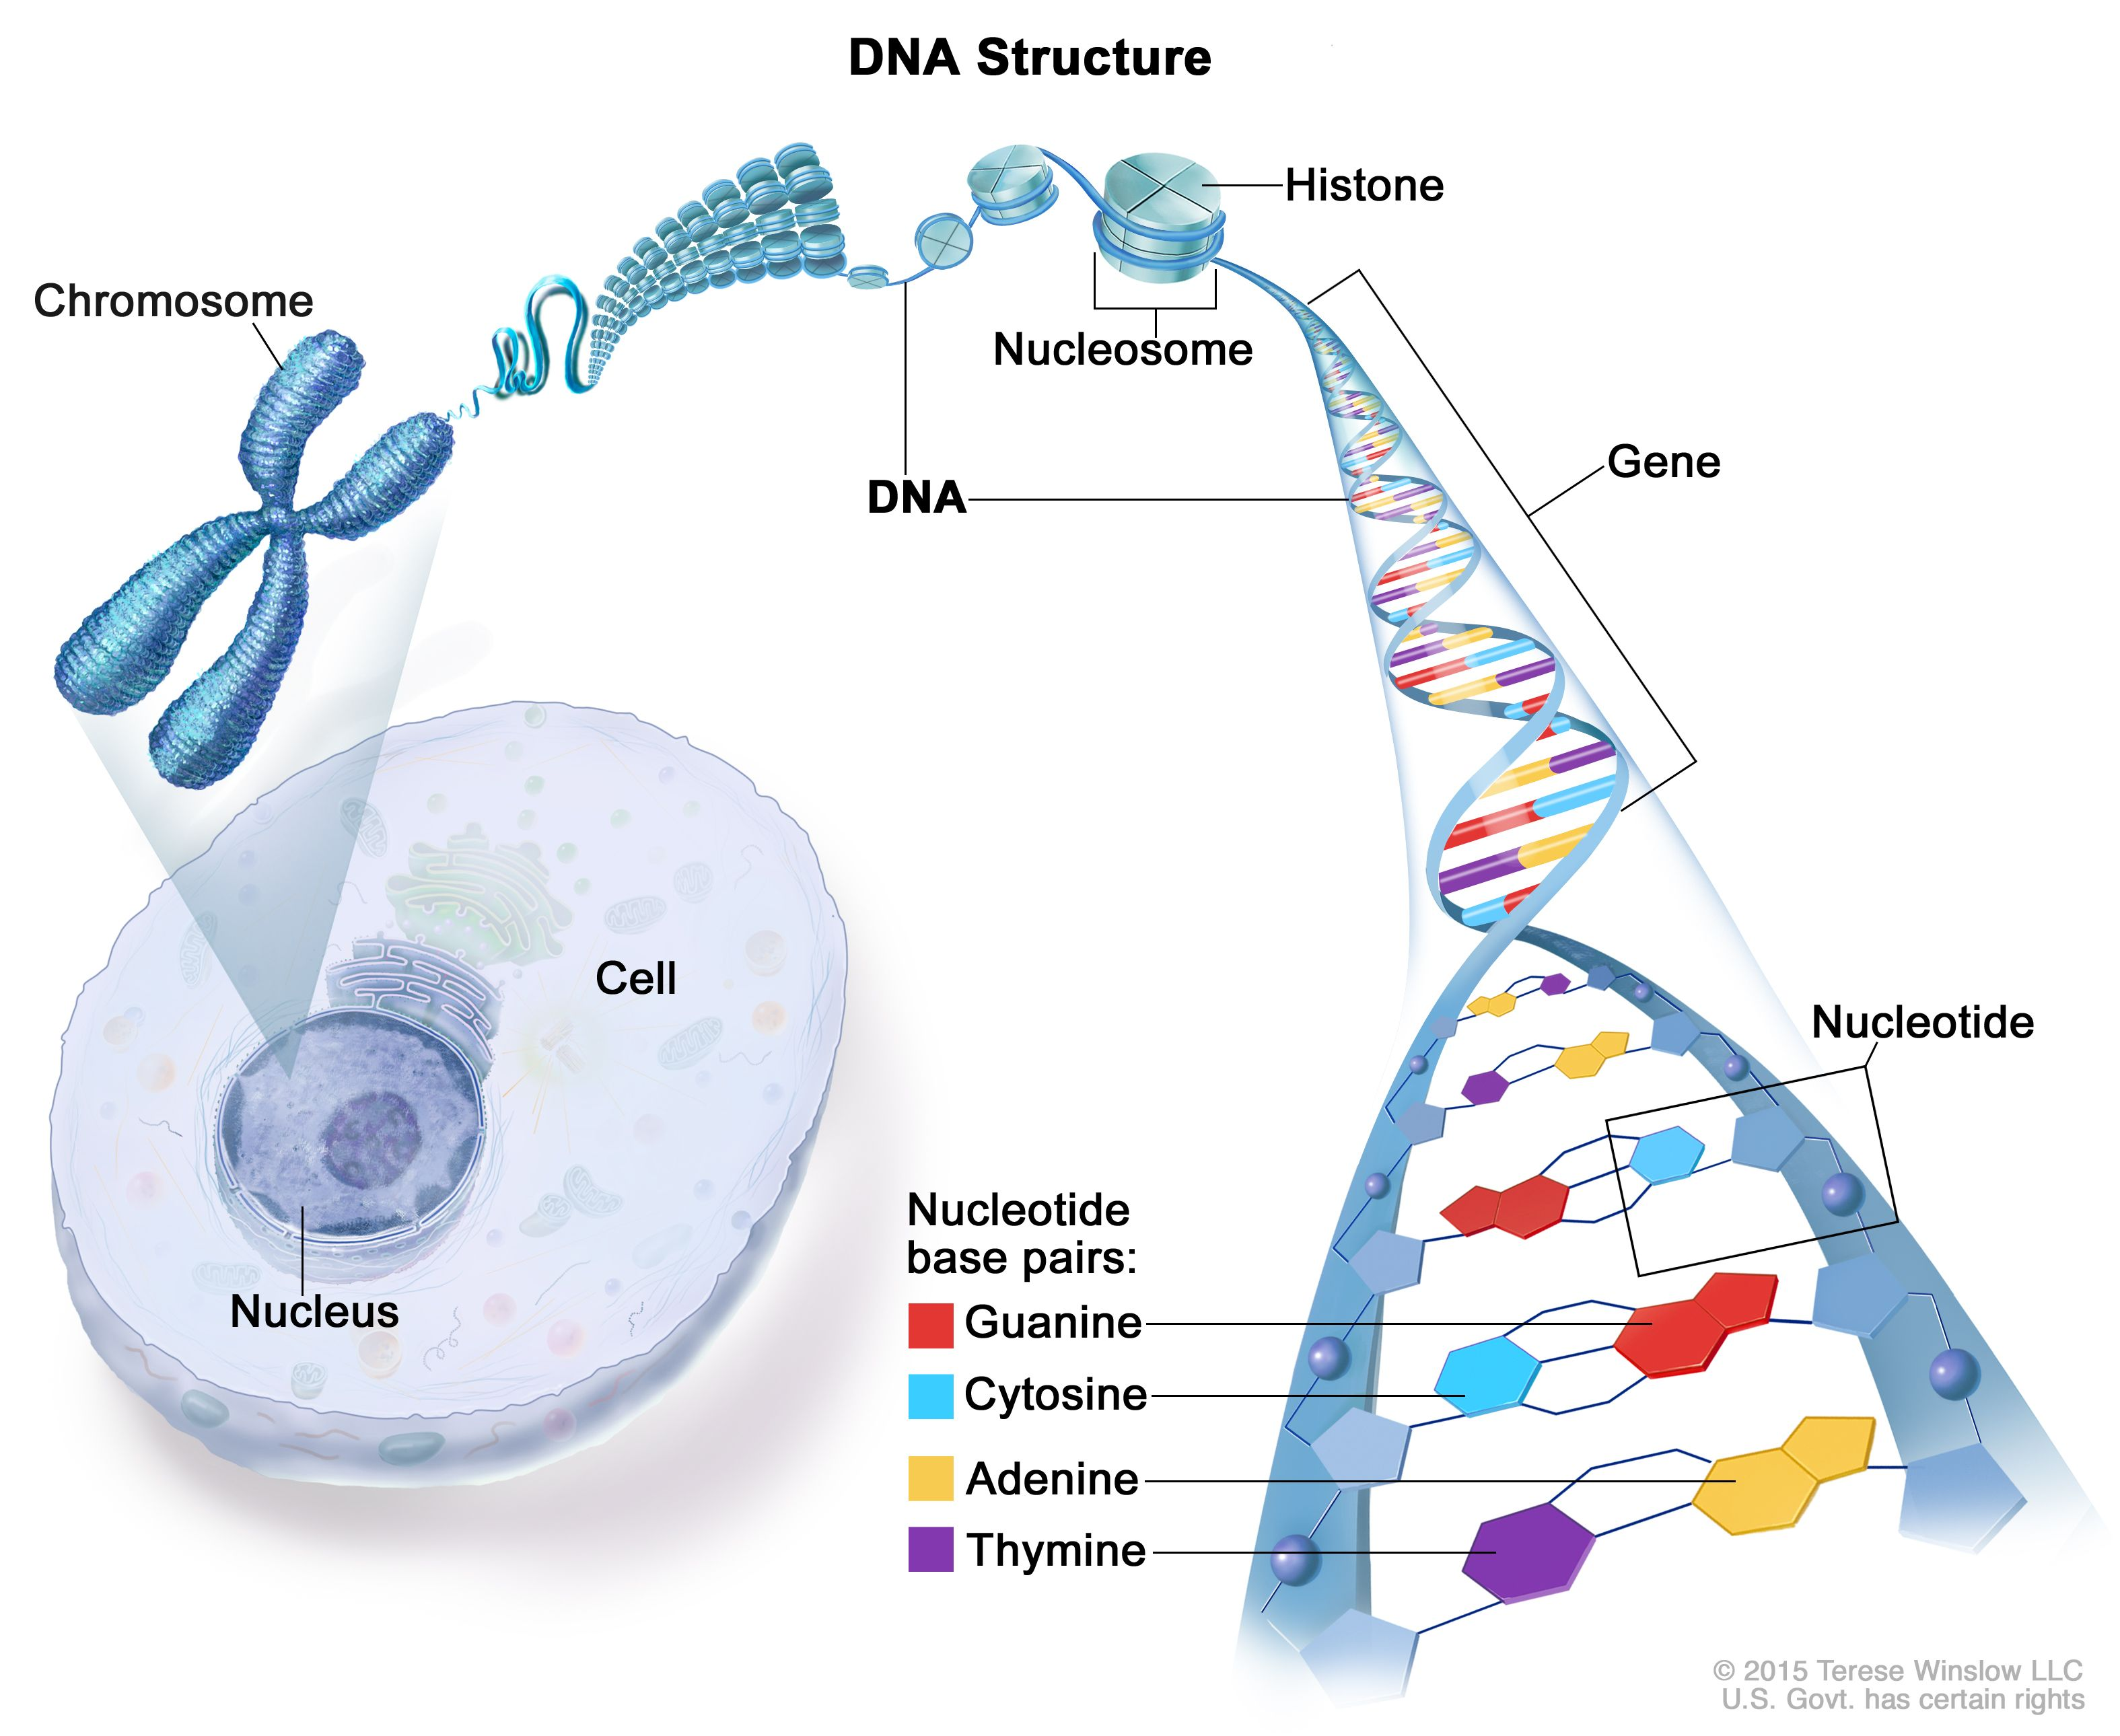
\includegraphics[width=\textwidth,height=0.65\textheight,keepaspectratio]{../img/neoantigen/dna}
			\label{img:mot2}
			\caption{Where DNA is located \cite{NCIdictionary2022}.}
		\end{figure}
	\end{frame}
	%-------------------------------------------------------
	%-------------------------------------------------------
	
	
	
	%-------------------------------------------------------
	%-------------------------------------------------------
	\begin{frame}{DNA}{De DNA a proteínas}
		\begin{figure}[]
			\centering
			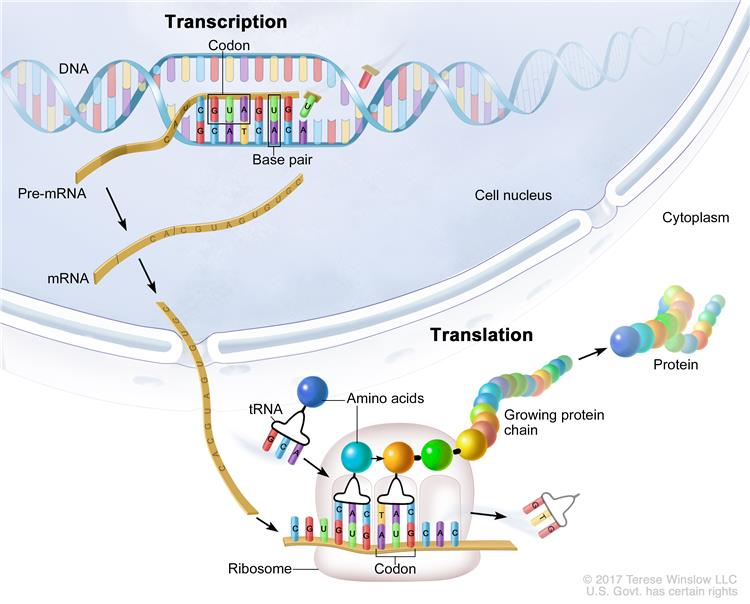
\includegraphics[width=0.7\textwidth]{../img/neoantigen/trans.jpg}
			\caption{Transcription and translation \cite{nci2020}.}
		\end{figure}
	\end{frame}
	%-------------------------------------------------------
	%-------------------------------------------------------
	
	%%%%%%%%%%%%%%%%%%%%%%%%%%%%%%%%%%%%%%%%%%%%%%%%%%%%%%%%%%%%%%%%%%%%%%%%%%%%%%%%%%%%%%%%%%%%%%%%%%%%%%%%%%%%%%%%
	%%%%%%%%%%%%%%%%%%%%%%%%%%%%%%%%%%%%%%%%%%%%%%%%%%%%%%%%%%%%%%%%%%%%%%%%%%%%%%%%%%%%%%%%%%%%%%%%%%%%%%%%%%%%%%%%
	%%%%%%%%%%%%%%%%%%%%%%%%%%%%%%%%%%%%%%%%%%%%%%%%%%%%%%%%%%%%%%%%%%%%%%%%%%%%%%%%%%%%%%%%%%%%%%%%%%%%%%%%%%%%%%%%
	\subsection{Mutaciones}
	%%%%%%%%%%%%%%%%%%%%%%%%%%%%%%%%%%%%%%%%%%%%%%%%%%%%%%%%%%%%%%%%%%%%%%%%%%%%%%%%%%%%%%%%%%%%%%%%%%%%%%%%%%%%%%%%
	%%%%%%%%%%%%%%%%%%%%%%%%%%%%%%%%%%%%%%%%%%%%%%%%%%%%%%%%%%%%%%%%%%%%%%%%%%%%%%%%%%%%%%%%%%%%%%%%%%%%%%%%%%%%%%%%
	%%%%%%%%%%%%%%%%%%%%%%%%%%%%%%%%%%%%%%%%%%%%%%%%%%%%%%%%%%%%%%%%%%%%%%%%%%%%%%%%%%%%%%%%%%%%%%%%%%%%%%%%%%%%%%%%

	%-------------------------------------------------------
	%-------------------------------------------------------
	\begin{frame}{Variantes y Mutaciones}{}
		\begin{figure}[h]
			\centering
			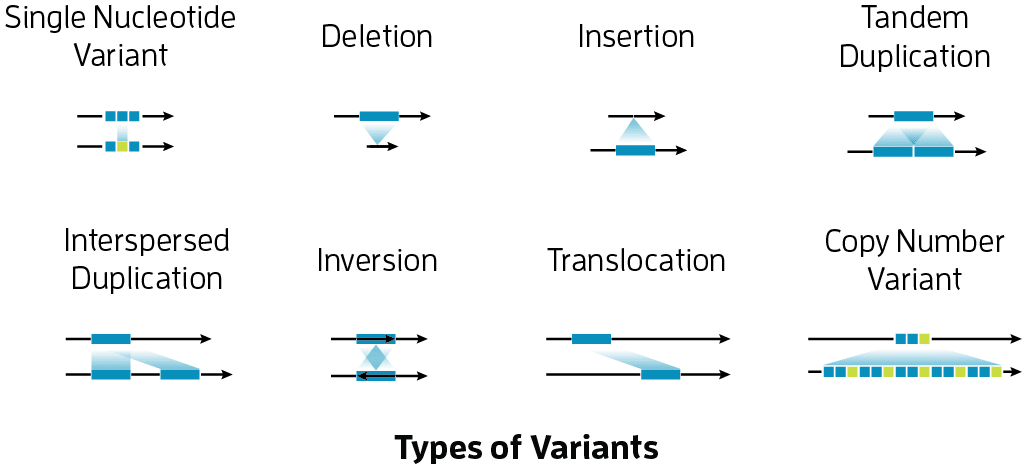
\includegraphics[width=\textwidth]{../img/neoantigen/variants}
			\caption{Example of structural variants. Source: \cite{sv_pacbio_2021}}
			\label{fig:variants}
		\end{figure}	
	\end{frame}
	%-------------------------------------------------------
	%-------------------------------------------------------

	
	%%%%%%%%%%%%%%%%%%%%%%%%%%%%%%%%%%%%%%%%%%%%%%%%%%%%%%%%%%%%%%%%%%%%%%%%%%%%%%%%%%%%%%%%%%%%%%%%%%%%%%%%%%%%%%%%
	%%%%%%%%%%%%%%%%%%%%%%%%%%%%%%%%%%%%%%%%%%%%%%%%%%%%%%%%%%%%%%%%%%%%%%%%%%%%%%%%%%%%%%%%%%%%%%%%%%%%%%%%%%%%%%%%
	%%%%%%%%%%%%%%%%%%%%%%%%%%%%%%%%%%%%%%%%%%%%%%%%%%%%%%%%%%%%%%%%%%%%%%%%%%%%%%%%%%%%%%%%%%%%%%%%%%%%%%%%%%%%%%%%
	\subsection{Neo antígenos}
	%%%%%%%%%%%%%%%%%%%%%%%%%%%%%%%%%%%%%%%%%%%%%%%%%%%%%%%%%%%%%%%%%%%%%%%%%%%%%%%%%%%%%%%%%%%%%%%%%%%%%%%%%%%%%%%%
	%%%%%%%%%%%%%%%%%%%%%%%%%%%%%%%%%%%%%%%%%%%%%%%%%%%%%%%%%%%%%%%%%%%%%%%%%%%%%%%%%%%%%%%%%%%%%%%%%%%%%%%%%%%%%%%%
	%%%%%%%%%%%%%%%%%%%%%%%%%%%%%%%%%%%%%%%%%%%%%%%%%%%%%%%%%%%%%%%%%%%%%%%%%%%%%%%%%%%%%%%%%%%%%%%%%%%%%%%%%%%%%%%%
	
	%-------------------------------------------------------
	%-------------------------------------------------------
	\begin{frame}{Inmunoterapia del Cáncer}{}		
		Es un tipo de tratamiento contra el Cáncer que estimula las defensas naturales del cuerpo para combatir el Cáncer \cite{inmunoterapy2022}.
		
		\begin{figure}
			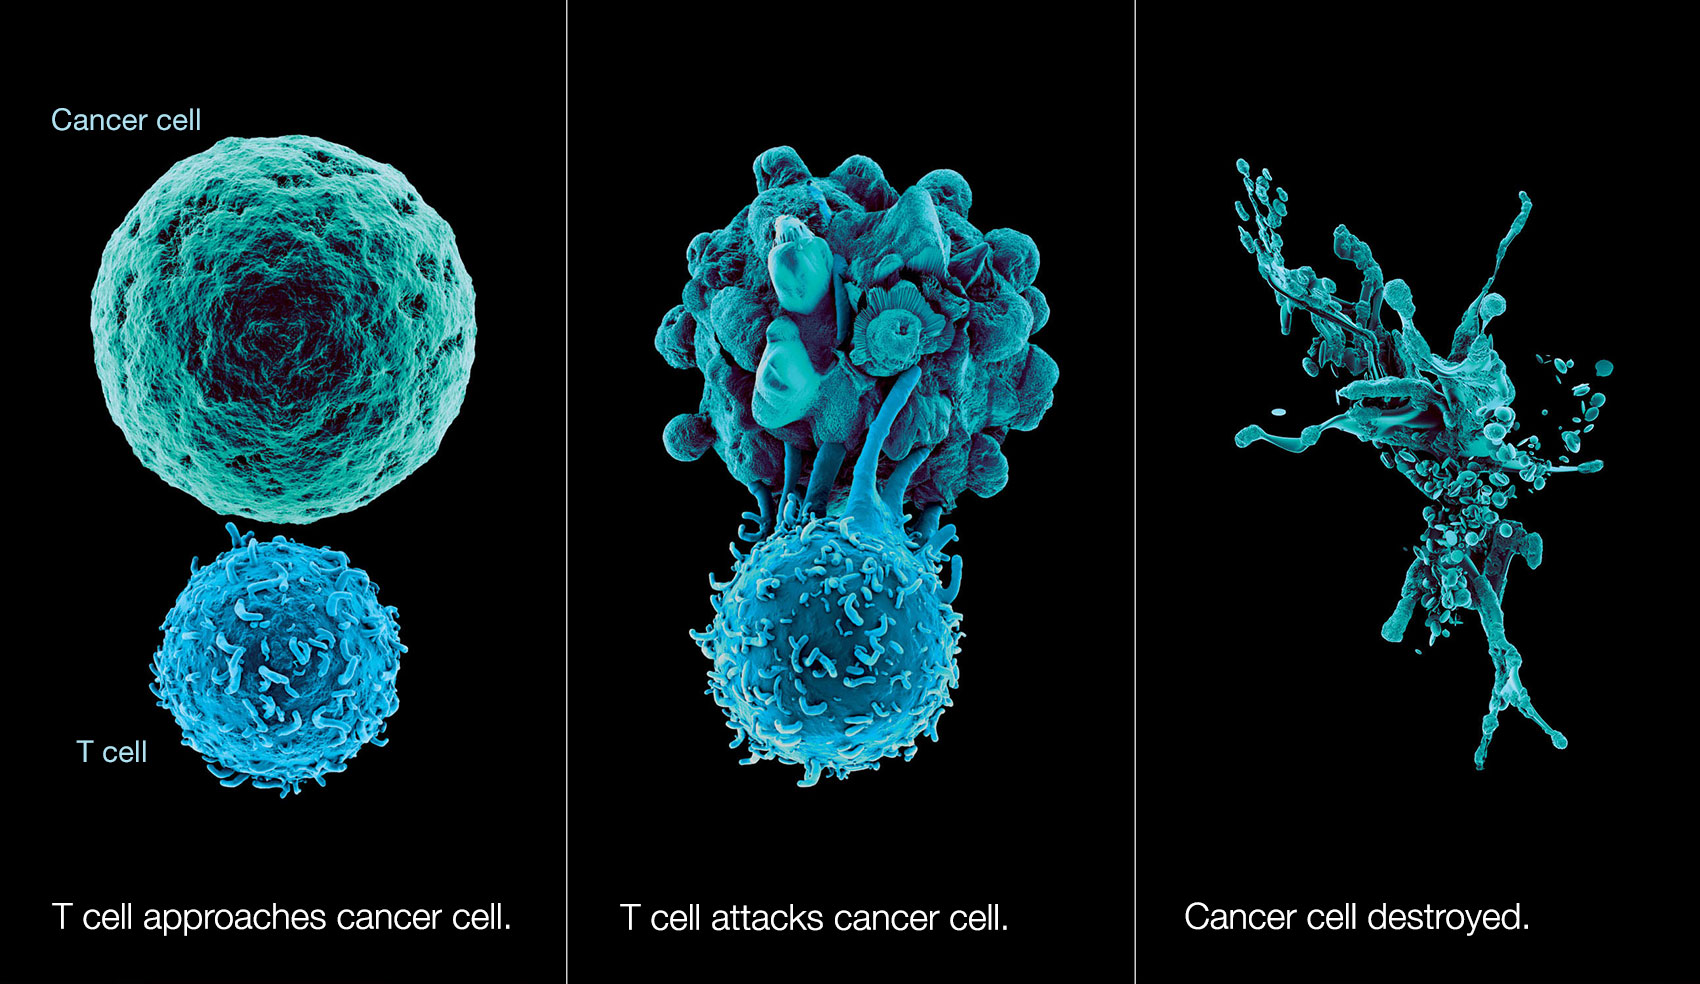
\includegraphics[width=0.85\textwidth]{../img/neoantigen/tcell}
			\caption{Ejemplo de como una célula T destruye células del cancer \cite{nortshore2022}.}
		\end{figure}		
	\end{frame}
	%-------------------------------------------------------
	%-------------------------------------------------------
	
	%-------------------------------------------------------
	%-------------------------------------------------------
	\begin{frame}{Inmunoterapia del Cáncer}{Neo antígenos}		
		\begin{block}{}
			Es una \textbf{proteína} que se forma en las células de Cáncer cuando ocurre mutaciones en el DNA, cumplen un rol importante al \textbf{estimular una respuesta inmune} \cite{NCIdictionary2022, borden2022cancer}.
		\end{block} 
		\begin{block}{}
			En la actualidad hay varios métodos para detectar a predecir neo antígenos, pero \textbf{solo una pequeña cantidad de ellos} logran estimular al sistema inmune \cite{chen2021challenges, hao2021improvement}.
		\end{block}
	\end{frame}
	%-------------------------------------------------------
	%-------------------------------------------------------
	
	%-------------------------------------------------------
	%-------------------------------------------------------
	\begin{frame}{MHC-I}{}		
		\begin{figure}[H]
			\centering
			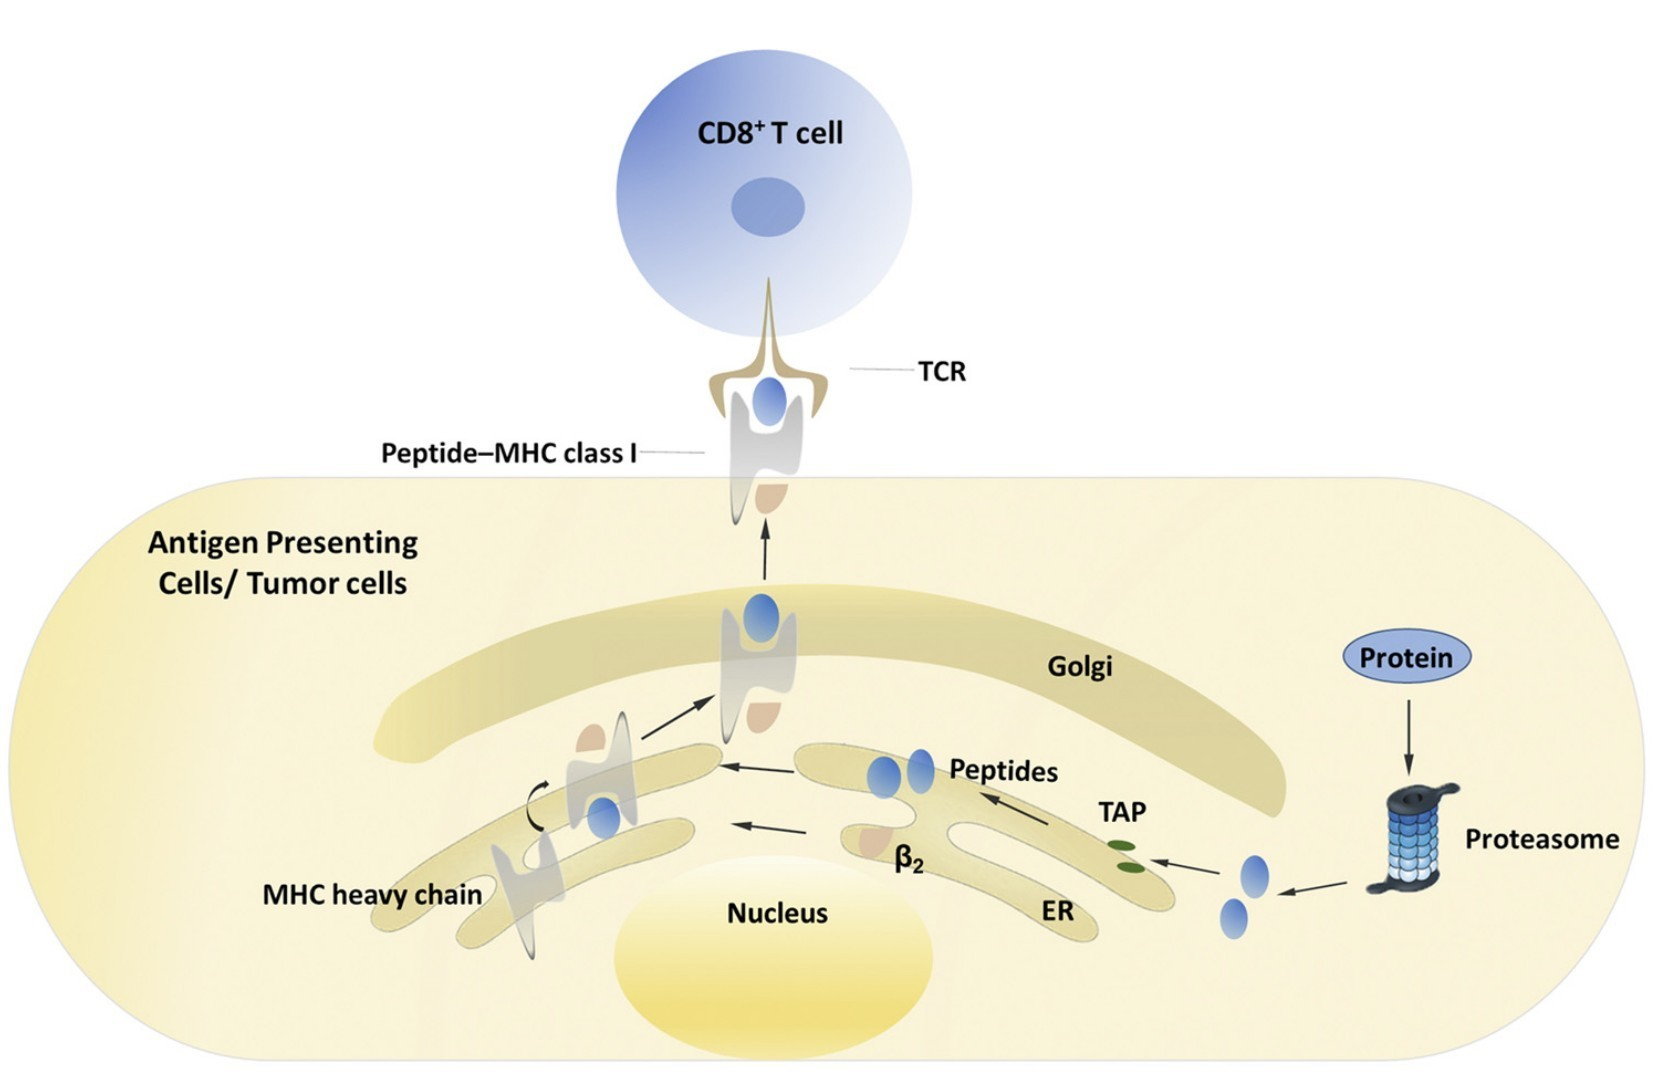
\includegraphics[width=0.9\textwidth]{../img/neoantigen/mhc1.jpg}
			\caption{Presentación de antígenos por MHC-I. Fuente: \cite{zhang2019application}}
			\label{fig:mhc1}
		\end{figure}	
	\end{frame}
	%-------------------------------------------------------
	%-------------------------------------------------------

	
	%-------------------------------------------------------
	%-------------------------------------------------------
	\begin{frame}{Inmunoterapia del Cáncer}{Generación de vacunas}	
		\begin{figure}
			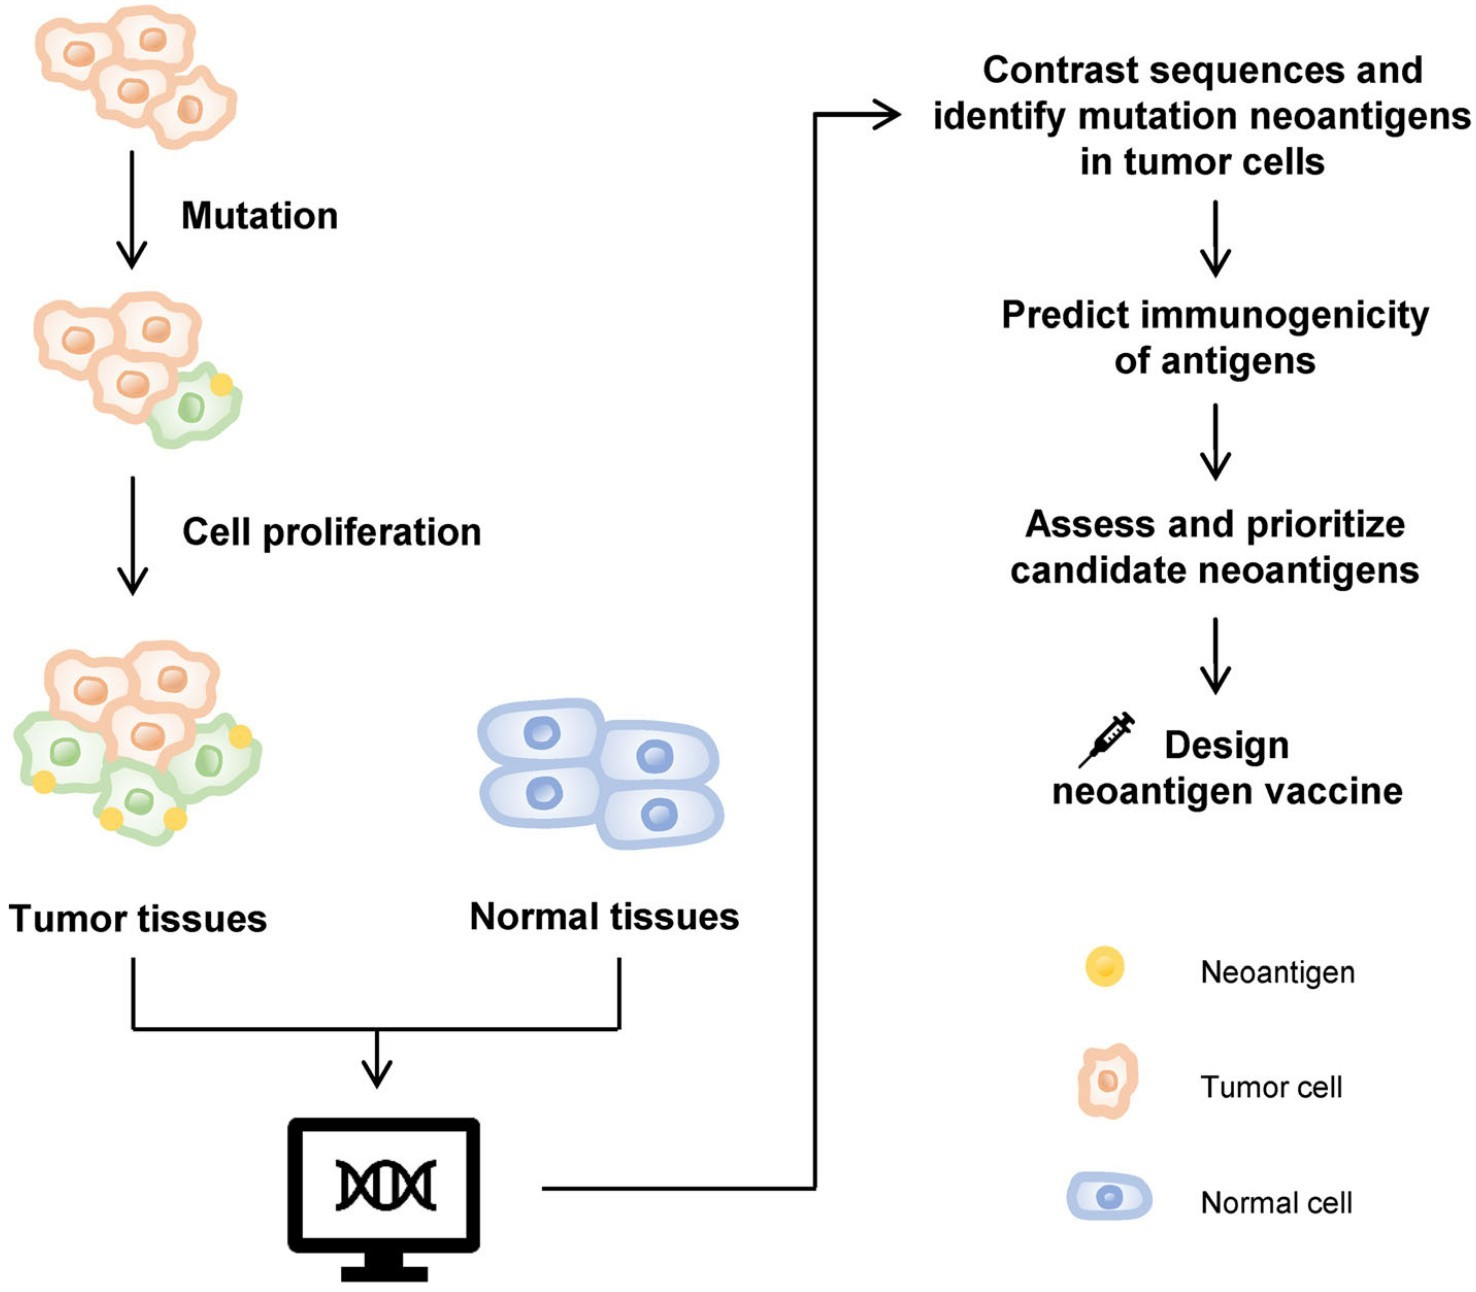
\includegraphics[width=0.6\textwidth]{../img/neoantigen/process}
			\caption{Proceso para la generación de vacunas personalizadas \cite{peng2019neoantigen}.}
		\end{figure}		
	\end{frame}
	%-------------------------------------------------------
	%-------------------------------------------------------
	
	
	%%%%%%%%%%%%%%%%%%%%%%%%%%%%%%%%%%%%%%%%%%%%%%%%%%%%%%%%%%%%%%%%%%%%%%%%%%%%%%%%%%%%%%%%%%%%%%%%%%%%%%%%%%%%%%%%
	%%%%%%%%%%%%%%%%%%%%%%%%%%%%%%%%%%%%%%%%%%%%%%%%%%%%%%%%%%%%%%%%%%%%%%%%%%%%%%%%%%%%%%%%%%%%%%%%%%%%%%%%%%%%%%%%
	%%%%%%%%%%%%%%%%%%%%%%%%%%%%%%%%%%%%%%%%%%%%%%%%%%%%%%%%%%%%%%%%%%%%%%%%%%%%%%%%%%%%%%%%%%%%%%%%%%%%%%%%%%%%%%%%
	\section{Problema y Objetivos}
	%%%%%%%%%%%%%%%%%%%%%%%%%%%%%%%%%%%%%%%%%%%%%%%%%%%%%%%%%%%%%%%%%%%%%%%%%%%%%%%%%%%%%%%%%%%%%%%%%%%%%%%%%%%%%%%%
	%%%%%%%%%%%%%%%%%%%%%%%%%%%%%%%%%%%%%%%%%%%%%%%%%%%%%%%%%%%%%%%%%%%%%%%%%%%%%%%%%%%%%%%%%%%%%%%%%%%%%%%%%%%%%%%%
	%%%%%%%%%%%%%%%%%%%%%%%%%%%%%%%%%%%%%%%%%%%%%%%%%%%%%%%%%%%%%%%%%%%%%%%%%%%%%%%%%%%%%%%%%%%%%%%%%%%%%%%%%%%%%%%%
	
	\subsection{Motivación y Problema}
	
	%-------------------------------------------------------
	%-------------------------------------------------------
	\begin{frame}{Motivación}{}	
		
		\begin{block}{}
			El cáncer representa el mayor problema de salud mundial, pero lamentablemente los métodos basados en cirugías, radioterapias, quimioterapias tienen baja efectividad \cite{peng2019neoantigen}.
		\end{block}	
		
		\begin{block}{}
			La inmunoterapia del cáncer es una alternativa para el desarrollo de vacunas personalizadas, pero este proceso depende de una correcta detección de neo antígenos \cite{de2020neoantigen, peng2019neoantigen}.
		\end{block}
		
	\end{frame}
	%-------------------------------------------------------
	%-------------------------------------------------------
	
	
	
	%-------------------------------------------------------
	%-------------------------------------------------------
	\begin{frame}{Problema}{}
		
		\begin{block}{}
			\textbf{Menos del 5\%} de los neoantígenos detectados logran activar a las células T (sistema inmune) \cite{de2020neoantigen, mill2022neoms, bulik2019deep, bassani2015mass, yadav2014predicting}. 
		\end{block}
		
	\end{frame}
	%-------------------------------------------------------
	%-------------------------------------------------------
	
	\subsection{Objetivo}
	
	%-------------------------------------------------------
	%-------------------------------------------------------
	\begin{frame}{Objetivos}{}	
		\begin{block}{}
			Desarrollar un método basado en \textit{deep learning} que mejore el acierto de la detección de neoantígenos a partir de la predicción del enlace pMHC.
		\end{block}
	
		\begin{block}{}
			Desarrollar una aplicación Web que permita realizar la predicción del enlace pMHC.
		\end{block}	
	\end{frame}
	%-------------------------------------------------------
	%-------------------------------------------------------
	

	
	%%%%%%%%%%%%%%%%%%%%%%%%%%%%%%%%%%%%%%%%%%%%%%%%%%%%%%%%%%%%%%%%%%%%%%%%%%%%%%%%%%%%%%%%%%%%%%%%%%%%%%%%%%%%%%%%
	%%%%%%%%%%%%%%%%%%%%%%%%%%%%%%%%%%%%%%%%%%%%%%%%%%%%%%%%%%%%%%%%%%%%%%%%%%%%%%%%%%%%%%
	\section{Propuesta}
	%%%%%%%%%%%%%%%%%%%%%%%%%%%%%%%%%%%%%%%%%%%%%%%%%%%%%%%%%%%%%%%%%%%%%%%%%%%%%%%%%%%%%%%%%%%%%%%%%%%%%%%%%%%%%%%%
	%%%%%%%%%%%%%%%%%%%%%%%%%%%%%%%%%%%%%%%%%%%%%%%%%%%%%%%%%%%%%%%%%%%%%%%%%%%%%%%%%%%%%%
	
	
	

	
	%-------------------------------------------------------
	%-------------------------------------------------------
	\begin{frame}{Propuesta}{}	
		\begin{figure}
			\centering
			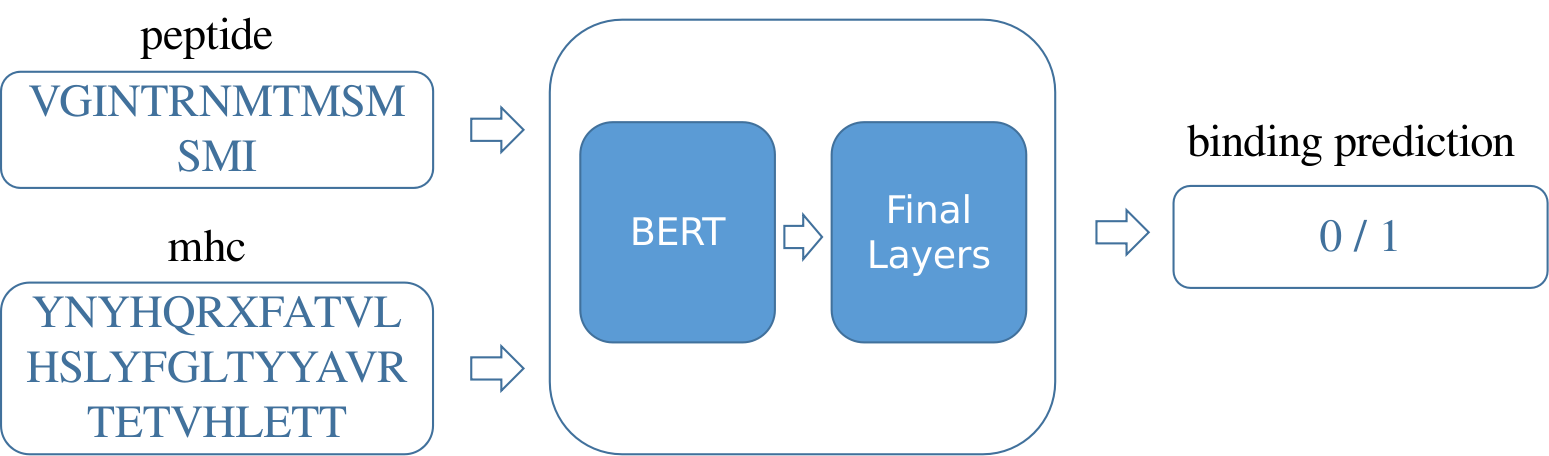
\includegraphics[width=0.5\textwidth]{../img/neoantigen/Picture2}	
			\caption{Propuesta}
		\end{figure}
	\end{frame}
	%-------------------------------------------------------
	%-------------------------------------------------------
	

	
	%%%%%%%%%%%%%%%%%%%%%%%%%%%%%%%%%%%%%%%%%%%%%%%%%%%%%%%%%%%%%%%%%%%%%%%%%%%%%%%%%%%%%%%%%%%%%%%%%%%%%%%%%%%%%%%%
	%%%%%%%%%%%%%%%%%%%%%%%%%%%%%%%%%%%%%%%%%%%%%%%%%%%%%%%%%%%%%%%%%%%%%%%%%%%%%%%%%%%%%%
	\section{Experimentos y Resultados}
	%%%%%%%%%%%%%%%%%%%%%%%%%%%%%%%%%%%%%%%%%%%%%%%%%%%%%%%%%%%%%%%%%%%%%%%%%%%%%%%%%%%%%%%%%%%%%%%%%%%%%%%%%%%%%%%%
	%%%%%%%%%%%%%%%%%%%%%%%%%%%%%%%%%%%%%%%%%%%%%%%%%%%%%%%%%%%%%%%%%%%%%%%%%%%%%%%%%%%%%%
	
	%-------------------------------------------------------
	%-------------------------------------------------------
	\begin{frame}{Protein Language Models}{}	
		\begin{table}[h]%
			\centering
			\scriptsize
			\caption{Pre-trainned BERT models for several protein tasks: TAPE, ProtBert, ESM1, and ESM-2.}%
			
			\label{tab:pretrained}
			
			\setlength{\tabcolsep}{0.5em} % for the horizontal padding
			{\renewcommand{\arraystretch}{1.1}% for the vertical padding
				\scriptsize
				\begin{tabular}{lllllll}
					
					\textbf{Model}   & \textbf{Dataset} & \textbf{Samples} & \textbf{Layers} & \textbf{Hidden size} & \textbf{Att. heads} & \textbf{Params.} \\ \hline
					
					TAPE             & Pfam             & 30M                   & 12              & 768                  & 12                       & 92M                 \\
					ProtBert-BFD     & BFD              & 2122M                 & 30              & 1024                 & 16                       & 420M                \\
					
					ProtT5-XL     & Uniref50, BFD              & 2122M                 & 24              & 1024                 & 32                       & 3B                \\
					
					ProtT5-XXL     & Uniref50, BFD              & 2122M                 & 24              & 1024                 & 128                       & 11B                \\
					
					
					
					ESM-1 (6 layers)  & Uniref50         & 60M                   & 6               & 768                  & 12                       & 43M                  \\
					ESM-1 (12 layers)  & Uniref50         & 60M                   & 12               & 768                  & 12                       & 85M                  \\
					ESM-1 (34 layers)  & Uniref50         & 60M                   & 34               & 1280                  & 20                       & 670M                  \\
					ESM-1b  & Uniref50         & 60M                   & 34               & 1280                  & 20                       & 650M                  \\
					
					ESM-2 (6 layers)  & Uniref50         & 60M                   & 6               & 320                  & 20                       & 8M                  \\
					ESM-2 (12 layers)  & Uniref50         & 60M                   & 12              & 480                  & 20                       & 35M                 \\
					ESM-2 (30 layers) & Uniref50         & 60M                   & 30              & 640                  & 20                       & 150M                \\
					ESM-2 (33 layers)  & Uniref50         & 60M                   & 33              & 1280                 & 20                       & 650M               \\
					
					ESM-2 (36 layers)  & Uniref50         & 60M                   & 36              & 2560                 & 20                       & 3B               \\
					
					ESM-2 (48 layers)  & Uniref50         & 60M                   & 48              & 5120                 & 20                       & 15B               \\
					
			\end{tabular}}
			
		\end{table}
		
	\end{frame}
	%-------------------------------------------------------
	%-------------------------------------------------------

	
	%-------------------------------------------------------
%-------------------------------------------------------
\begin{frame}{Hiperparámetros}{}
	\begin{table}[]
		\centering
		\caption{Hyper-parameters configuration used to train ESM2 models in order to evaluate if they got into vanishing gradient problem.}
		\label{tab:configurations}
		
		\begin{tabular}{lllll} 
			\textbf{Configuration} & \textbf{lr}            & \textbf{Epochs} & \textbf{Warmup steps} & \textbf{Batch size}       \\ \hline
			c1 & 4e-4 & 6 & 2000 & 16 \\
			c2 & 4e-4 & 6 & 2000 & 8 \\
			c3 & 2e-5 & 6 & 2000 & 16 \\
			c4 & 1e-5 & 30 & 101066 & 16 \\
			c5 & 2e-6 & 60 & 202132 & 16 \\
			
		\end{tabular}
	\end{table}
\end{frame}
%-------------------------------------------------------
%-------------------------------------------------------

%-------------------------------------------------------
%-------------------------------------------------------
\begin{frame}{Experimentos}{}
	\begin{enumerate}
		\item Evaluar las configuraciones de hiperparámetros al hacer fine-tuning a los modelos ESM2.
		\item Comparar el desempeño de LoRA, distillation y un método de congelamiento de capas.
		\item Comparar el desempeño de los pLMs: TAPE, ProdBert-BFD y ESM2 para la tarea de pMHC.
		\item Comparar el mejor modelo de los experimentos anteriores con los métodos del estado del arte.
	\end{enumerate}
\end{frame}
%-------------------------------------------------------
%-------------------------------------------------------
	
	%-------------------------------------------------------
	%-------------------------------------------------------
	\begin{frame}{Resultados}{}
		\begin{table}[]
			\centering
			\caption{Resultados obtenidos en cada base de datos. }
			\label{tab:results}
			\setlength{\tabcolsep}{0.8em} % for the horizontal padding
			{\renewcommand{\arraystretch}{1.3}% for the vertical padding
				\begin{tabular}{lllll}
					\hline
					\textit{\textbf{Allele}} & \textit{\textbf{Accuracy}} & \textit{\textbf{F1 score}} & \textit{\textbf{Precision}} & \textit{\textbf{Recall}} \\
					\hline
					A*01:01                  & 0.978                      & 0.917                      & 0.982                       & 0.887                    \\
					A*0201                   & 0.962                      & 0.956                      & 0.965                       & 0.948                    \\
					A*02:03                  & 0.992                      & 0.979                      & 0.994                       & 0.969                    \\
					A*31:01                  & 0.980                      & 0.968                      & 0.989                       & 0.951                    \\
					B*44:02                  & 0.991                      & 0.981                      & 0.968                       & 0.997                    \\
					B*44:03                  & 0.992                      & 0.987                      & 0.995                       & 0.980                   
				\end{tabular}
			}
		\end{table}
	\end{frame}
	%-------------------------------------------------------
	%-------------------------------------------------------
	
	%-------------------------------------------------------
	%-------------------------------------------------------
	\begin{frame}{Resultados}{}
		\begin{table}[h]
			\centering
			\caption{AUC entre la propuesta, BERTMHC, NetMHCpan3.2, PUFFIN y MHCnuggets.}
			\setlength{\tabcolsep}{0.8em} % for the horizontal padding
			{\renewcommand{\arraystretch}{1.3}% for the vertical padding
				\begin{tabular}{lc}
					\hline
					\textbf{Modelo} & \textbf{AUC} \\ \hline
					Propuesta & 0.73\\
					BERTMHC & 0.72\\
					NetMHCpan3 & 0.68\\
					PUFFIN & 0.69\\
					MHCnuggets & 0.58\\
				\end{tabular}
			}
		\end{table}
	\end{frame}
	%-------------------------------------------------------
	%-------------------------------------------------------
	
	
	%%%%%%%%%%%%%%%%%%%%%%%%%%%%%%%%%%%%%%%%%%%%%%%%%%%%%%%%%%%%%%%%%%%%%%%%%%%%%%%%%%%%%%%%%%%%%%%%%%%%%%%%%%%%%%%%
	%%%%%%%%%%%%%%%%%%%%%%%%%%%%%%%%%%%%%%%%%%%%%%%%%%%%%%%%%%%%%%%%%%%%%%%%%%%%%%%%%%%%%%
	\section{Conclusiones}
	%%%%%%%%%%%%%%%%%%%%%%%%%%%%%%%%%%%%%%%%%%%%%%%%%%%%%%%%%%%%%%%%%%%%%%%%%%%%%%%%%%%%%%%%%%%%%%%%%%%%%%%%%%%%%%%%
	%%%%%%%%%%%%%%%%%%%%%%%%%%%%%%%%%%%%%%%%%%%%%%%%%%%%%%%%%%%%%%%%%%%%%%%%%%%%%%%%%%%%%%
	
	
	%-------------------------------------------------------
	%-------------------------------------------------------
	\begin{frame}{Conclusiones}{}
		\begin{block}{}
			En esta investigación se propuso el uso de un modelo \textit{transformer} ya entrenado con una base de datos de 30 millones de proteínas. Luego, esta red fue conectada de forma paralela con una red CNN.
		\end{block}
		
		\begin{block}{}
			El uso de \textit{transfer learning} es una buena opción para suplir la falta de muestras en ciertos problemas y reducir el tiempo de entrenamiento.		
		\end{block}
		
		\begin{block}{}
			La propuesta llego a mejorar los mejores métodos de detección de afinidad entre un péptido y una proteína MHC-II. Como trabajo futuro, se planteará la misma propuesta para proteínas MHC-I.	
		\end{block}
		
		\begin{block}{}
			Predecir la afinidad entre un péptido y una proteína MHC, es uno de los paso mas importantes par calificar al péptido como un neo antígeno, capaz de generar una respuesta inmunitaría.
		\end{block}
	\end{frame}
	%-------------------------------------------------------
	%-------------------------------------------------------
	
	%%%%%%%%%%%%%%%%%%%%%%%%%%%%%%%%%%%%%%%%%%%%%%%%%%%%%%%%%%%%%%%%%%%%%%%%%%%%%%%%%%%%%%%%%%%%%%%%%%%%%%%%%%%%%%%%
	%%%%%%%%%%%%%%%%%%%%%%%%%%%%%%%%%%%%%%%%%%%%%%%%%%%%%%%%%%%%%%%%%%%%%%%%%%%%%%%%%%%%%%
	\section{Trabajos futuros}
	%%%%%%%%%%%%%%%%%%%%%%%%%%%%%%%%%%%%%%%%%%%%%%%%%%%%%%%%%%%%%%%%%%%%%%%%%%%%%%%%%%%%%%%%%%%%%%%%%%%%%%%%%%%%%%%%
	%%%%%%%%%%%%%%%%%%%%%%%%%%%%%%%%%%%%%%%%%%%%%%%%%%%%%%%%%%%%%%%%%%%%%%%%%%%%%%%%%%%%%%
	
	
	%-------------------------------------------------------
	%-------------------------------------------------------
	\begin{frame}{Trabajos futuros}{}
		\begin{block}{}
			Recientemente un trabajo \cite{hashemi2022improved} tambien propone el uso de \textit{transfer learning} pero de un modelo pre-entrenado con 250 millones de proteínas. Entonces, se plantea utilizar la misma red, aumentar la cantidad de muestras y evaluar los resultados.
		\end{block}
		
		\begin{block}{}
			Actualmente se cuenta con una base de datos de proteínas MHC \cite{e2019phla3d}, entonces utilizando AlphaFold de Google, se plantea predecir la estructura de varios péptidos y analizar el enlace péptido-MHC desde un punto de vista de la computación gráfica.	
		\end{block}
		
		
	\end{frame}
	%-------------------------------------------------------
	%-------------------------------------------------------
	
	%-------------------------------------------------------
	%-------------------------------------------------------
	\begin{frame}[allowframebreaks]
		\frametitle{References}
		%\bibliographystyle{amsalpha}
		\bibliographystyle{IEEEtran}
		\bibliography{../bibliography_thesis.bib}
	\end{frame}
	%-------------------------------------------------------
	%-------------------------------------------------------
	
	%-------------------------------------------------------
	%-------------------------------------------------------
	\if\mycmd1 % MY THEME
	\1{
		{\1
			\begin{frame}[plain,noframenumbering]
				%\finalpage{Thank you}
				\begin{figure}[]
					\centering
					
\includegraphics[width=\textwidth,height=0.7\textheight,keepaspectratio]{../img/question.png}
					%\label{img:mot2}
					%\caption{Image example in 2 gray levels.}
				\end{figure}
		\end{frame}}
		\else % CS THEME
		\begin{frame}{Questions?}
			\begin{figure}[]
				\centering
				
\includegraphics[width=\textwidth,height=0.7\textheight,keepaspectratio]{../img/question.png}
				%\label{img:mot2}
				%\caption{Image example in 2 gray levels.}
			\end{figure}
			
		\end{frame}
		\fi
		%-------------------------------------------------------
		%-------------------------------------------------------
		
		
	\end{document}